\documentclass[11pt]{beamer}
\usetheme{Dresden}
%\usecolortheme{beaver}
\usepackage[utf8]{inputenc}
\usepackage{amsmath}
\usepackage{amsfonts}
\usepackage{amssymb}
\usepackage{graphicx}
\usepackage{listings}
\usepackage{verbatim}
\author{Zheng Zheng}
\title{Topic 9 - Makefiles, Testing and Static Analysis}
%\setbeamercovered{transparent} 
%\setbeamertemplate{navigation symbols}{} 
%\logo{} 
\institute{McMaster University} 
\date{Winter 2023} 
\subject{COMPSCI 1XC3 - Computer Science Practice and Experience: Development Basics} 
\stepcounter{section}

\definecolor{mGreen}{rgb}{0,0.6,0}
\definecolor{mGray}{rgb}{0.5,0.5,0.5}
\definecolor{mPurple}{rgb}{0.58,0,0.05}
\definecolor{mGreen2}{rgb}{0.05,0.65,0.05}
\definecolor{mGray2}{rgb}{0.55,0.55,0.55}
\definecolor{mPurple2}{rgb}{0.63,0.05,0.05}
\definecolor{backgroundColour}{rgb}{0.95,0.95,0.92}
\definecolor{backgroundColour2}{rgb}{0.95,0.92,0.95}

\lstdefinestyle{C}{
    backgroundcolor=\color{backgroundColour},   
    commentstyle=\color{mGreen},
    keywordstyle=\color{blue},
    numberstyle=\tiny\color{mGray},
    stringstyle=\color{mPurple},    
    basicstyle=\footnotesize,
    breakatwhitespace=false,         
    breaklines=true,                 
    captionpos=b,                    
    keepspaces=true,                 
    numbers=left,                    
    numbersep=5pt,                  
    showspaces=false,                
    showstringspaces=false,
    showtabs=false,                  
    tabsize=2,
    language=C
}

\definecolor{t_comment}{rgb}{0.2,1,0.2}
\definecolor{t_mGray}{rgb}{0.5,0.5,0.5}
\definecolor{t_mPurple}{rgb}{0.58,0,0.05}
\definecolor{t_blue}{rgb}{0.4,0.6,0.8}
\definecolor{t_mGreen2}{rgb}{0.05,0.65,0.05}
\definecolor{t_mGray2}{rgb}{0.75,0.75,0.75}
\definecolor{t_mPurple2}{rgb}{0.63,0.05,0.05}
\definecolor{t_bg}{rgb}{0.15,0.15,0.18}

\lstdefinestyle{terminal}{
    backgroundcolor=\color{t_bg},   
    commentstyle=\color{t_comment},
    keywordstyle=\color{t_blue},
    numberstyle=\tiny\color{t_mGray},
    stringstyle=\color{t_mGray2}, 
    basicstyle=\footnotesize\color{t_mGray2},
    breakatwhitespace=false,         
    breaklines=true,                 
    captionpos=b,                    
    keepspaces=true,                 
    numbers=none,                    
    numbersep=5pt,                  
    showspaces=false,                
    showstringspaces=false,
    showtabs=false,                  
    tabsize=2,
    language=bash
}

\definecolor{eggplant}{rgb}{0.52,0.11,0.3}

\usecolortheme[named=eggplant]{structure}

\begin{document}

\begin{frame}
\center
COMPSCI 1XC3 - Computer Science Practice and Experience:
Development Basics
\titlepage
% Toggle for C chapters
% Adapted from C: How to Program 8th ed., Deitel \& Deitel
\end{frame}

\begin{frame}
\tableofcontents
\end{frame}

\section[Compilation]{Reviewing Compilation}
\begin{frame}{Stages of Compilation}
Recall the stages of compilation: \\
\begin{columns}
\begin{column}{0.4\textwidth}
\begin{itemize}
\item Preprocessor directives (\texttt{include} and \texttt{define} etc) are resolved.
\item Parsing \& AST generation
\item Assembly of object (machine) code 
\item Linking with other object files (if applicable).
\end{itemize}
\end{column}
\begin{column}{0.6\textwidth}
\includegraphics[scale=0.40]{stages.png}
\end{column}
\end{columns}
\end{frame}

\begin{frame}{Object Files}
So what's the point of object files? 
\begin{itemize}
\item An object file is machine code that was compiled from it's source code file, but \emph{without} the code for any called functions in other source code files. 
\item Instead, object files contain \emph{links to} the needed functions in the needed files and libraries.   
\item Object files are binary encoded, not character encoded, so there's no point trying to look at them with \texttt{cat} or \texttt{less}.  
\end{itemize}
By compiling an object file for each source code file \emph{separately}, the object files only need to be updated \emph{if the source code is updated!}  This can produce a massive speed boost in compilation time!  \\
\end{frame}

\begin{frame}[fragile=singleslide]{OBJECTion!!!}
Using object files correctly requires effort.  We can compile a batches of source code files to object files using glob patterns and the \texttt{-c} flag:
\begin{lstlisting}[style=terminal]
$ gcc -c *.c
\end{lstlisting}
But then when we go to compile our program from object code:
\begin{lstlisting}[style=terminal]
$ gcc -o main main.c lib1.o lib2.o lib3.o etc.o 
\end{lstlisting}
We have to manually include our object files, which is tedious and time consuming. So we're saving compilation time, but losing time to longer commands.\\ 
\vspace{1em}
\center
\textbf{There has to be a better way!} \\
\end{frame}

\section[Makefiles]{Makefiles: An Introduction}
\begin{frame}{\texttt{make} me a sandwich!}
\texttt{make} is a program which automates the compilation process.
\begin{itemize}
\item \texttt{make} compiles only those source code files that \textbf{need} to be recompiled to produce the executable.
\item It does this by checking the time at which your source code files were last saved, and the time when the program was last compiled.
\item \texttt{make} requires a special configuration file, called a \texttt{makefile}, which tells it which files to compile, which compiler to use, etc.
\end{itemize}
\vspace{1em}
\center
Makefiles are \emph{not} Bash Scripts.  
\end{frame}

\begin{frame}[fragile=singleslide]{sudo \texttt{make} me a sandwich!}
Makefiles are composed of \textbf{rules}.
\begin{lstlisting}[style=terminal]
<target> : <prerequisites>
	<recipe>
\end{lstlisting}
\begin{itemize}
\item A \texttt{target} can be one of three things:
\begin{itemize}
\item An executable file
\item An object file
\item A ``Phony Target'', which functions as a special command (i.e, \texttt{clean}). 
\end{itemize}
\item A \texttt{prerequisites} are the files that are used as input to create the target.  
\item A \texttt{recipe} is a Bash command that \texttt{make} performs to create the target.  
\end{itemize}
Each recipe line must be started with a \textbf{tab} (\texttt{\textbackslash t}) character.  Spaces are invalid syntax!
\end{frame}

\begin{frame}[fragile=singleslide]{A Simple Example}
Recall the files we used in Lab 6 to create static and dynamic libraries.  
\center
\includegraphics[scale=0.5]{filegraph.png} \\
\flushleft
We used lots of fancy compilation methods to create static and dynamic libraries, but you can also compile these using more simple invocations of gcc, such as 
\begin{lstlisting}[style=terminal]
$ gcc -Wall -o top top.c sums.o products.o C_Shanties.o
\end{lstlisting}
\end{frame}

\begin{frame}[fragile=singleslide]{Makefile-ification}
If we write rules to produce all the object files and the final executable into a makefile, we would get the following: 
\begin{lstlisting}[style=terminal]
top : top.c sums.o products.o C_Shanties.o 
	gcc -Wall -o top top.c sums.o products.o C_Shanties.o

C_Shanties.o : C_Shanties.c
	gcc -Wall -c -o C_Shanties.o C_Shanties.c

products.o : products.c
	gcc -Wall -c -o products.o products.c

sums.o : sums.c
	gcc -Wall -c -o sums.o sums.c
\end{lstlisting}
\end{frame}

\begin{frame}[fragile=singleslide]{How to use \texttt{make}}
Now that we have our makefile in place, we can start compiling!  To compile the ``default goal'', simply type:
\begin{lstlisting}[style=terminal]
$ make
\end{lstlisting}
To compile any of the targets in the file, just specify the target:
\begin{lstlisting}[style=terminal]
$ make sums.o
$ make top
\end{lstlisting}
To invoke a phony target, again, just type the name:
\begin{lstlisting}[style=terminal]
$ make cleanup
\end{lstlisting}
{\center
\emph{Nothing could be more simple!}}
\end{frame}

\begin{frame}{So how does this Work?}
\begin{itemize}
\item On a default invokation (i.e., just calling \texttt{make} with no arguments), \texttt{make} will use the first rule as its compilation target.  
\begin{itemize}
\item Therefore, your top file should be at the top! 
\end{itemize}
\item Whether the target is default or specified, \texttt{make} recursively (!) processes the rules for all prerequisites of the target rule.  
\item If the source file is newer than its corresponding object file, or if the object file doesn't exist, \texttt{make} will produce it.
\begin{itemize}
\item For testing purposes, \texttt{touch} updates the timestamp on a file without modifying the contents.
\end{itemize}
\item Any object file which needs to be linked to other object files will be regenerated as well, if any of the object files it needs are newer than itself.  
\end{itemize}
\end{frame}

\section[Variables]{Using Variables in Makefiles}
\begin{frame}{Variables!}
\center
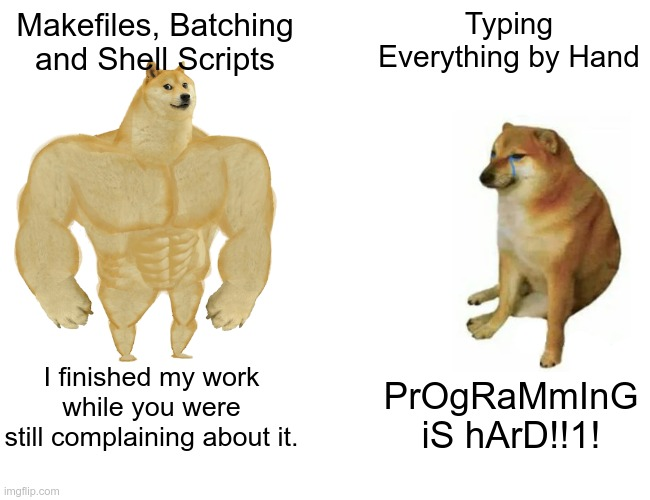
\includegraphics[scale=0.3]{scripting.jpg}
\end{frame}

\begin{frame}{Variables $<$3}
As with so many things in life, we can make things once again simpler in the long term by complicating things in the short term.  
\begin{itemize}
\item Makefiles support variables which are similar in many ways to the variables in shell scripting.  
\item Variables once again need the variable substitution operator \texttt{\$()} to work.
\begin{itemize}
\item This time, enclosing the variable name in round braces is considered good etiquette.  
\end{itemize}
\item You also don't have to worry about not leaving some whitespace this time around.  (But don't go overboard).
\end{itemize}
When set up correctly, variables let control many things about our compilation processes from a few lines at the top of the file.  
\end{frame}

\begin{frame}[fragile=singleslide]{Abstract Out the Compiler!}
\begin{lstlisting}[style=terminal]
CC = gcc

top : top.c sums.o products.o C_Shanties.o 
	$(CC) -Wall -o top top.c sums.o products.o C_Shanties.o

C_Shanties.o : C_Shanties.c
	$(CC) -Wall -c -o C_Shanties.o C_Shanties.c

products.o : products.c
	$(CC) -Wall -c -o products.o products.c

sums.o : sums.c
	$(CC) -Wall -c -o sums.o sums.c
\end{lstlisting}
\end{frame}

\begin{frame}[fragile=singleslide]{Abstract Out the Compiler Flags!}
\begin{lstlisting}[style=terminal]
CC = gcc
Cflags = -Wall -o 

top : top.c sums.o products.o C_Shanties.o 
	$(CC) $(Cflags) top top.c sums.o products.o C_Shanties.o

C_Shanties.o : C_Shanties.c
	$(CC) -c $(Cflags) C_Shanties.o C_Shanties.c

products.o : products.c
	$(CC) -c $(Cflags) products.o products.c

sums.o : sums.c
	$(CC) -c $(Cflags) sums.o sums.c
\end{lstlisting}
\end{frame}

\begin{frame}[fragile=singleslide]{Abstract Out the List of Objects!}
\begin{lstlisting}[style=terminal, language=bash]
CC = gcc
Cflags = -Wall -o 
objects = sums.o products.o C_Shanties.o 

top : top.c $(objects)
	$(CC) $(Cflags) top top.c $(objects)

C_Shanties.o : C_Shanties.c
	$(CC) -c $(Cflags) C_Shanties.o C_Shanties.c

products.o : products.c
	$(CC) -c $(Cflags) products.o products.c

sums.o : sums.c
	$(CC) -c $(Cflags) sums.o sums.c
	
# Makefile Comments Use Octothorpe BTW!
\end{lstlisting}
\end{frame}

\begin{frame}[fragile=singleslide]{\texttt{clean} up your Act!}
Although it isn't required, it is conventional to include a ``cleanup'' phony target, which deletes files used during executable generation, but which are not needed afterwards.  
\begin{lstlisting}[style=terminal]
clean : 
	rm -f $(objects)
\end{lstlisting}
\begin{itemize}
\item Specifying no prerequisites makes this a ``stand alone'' rule.
\item The \texttt{-f} flag on \texttt{rm} means ``force''.  It stops \texttt{rm} complaining about requests to delete non-existent files.
\end{itemize}
\end{frame}

\begin{frame}[fragile=singleslide]{\texttt{all} in the Family}
Another phony target typically included is ``all''.  This isn't necessary unless a makefile has more than one final target (i.e., if there was more than one top file that could have gone in the top slot).  
\begin{lstlisting}[style = terminal, language=bash]
all_targets = executable1 executable2 executable3

all : $(all_targets)
# No recipe! 
\end{lstlisting}
The ``all'' rule typically doesn't do anything by itself, it just queues up all valid final targets for regeneration by making them prerequisites.  
\end{frame}

\section[Testing]{Automated Testing using \texttt{diff}}
\begin{frame}{This is Why We Test Things!}
Automating things is both efficient and satisfying, so let's automate one of the more tedious programming tasks: \textbf{testing}!
\begin{itemize}
\item When testing a program, we compare the \textbf{expected output} of our program to the \textbf{actual output}.
\item Of course, this only works if both outputs were produced from the same \textbf{input}.
\item The expected output can be generated by a number of processes:
\begin{itemize}
\item Human design
\item A different, perhaps less efficient algorithm 
\item Customer Requirements
\end{itemize}
\end{itemize}
\end{frame}

\begin{frame}[fragile=singleslide]{\texttt{diff}erent Strokes for \texttt{diff}erent Folks!}
\begin{columns}
\begin{column}{0.5\textwidth}
\center
\texttt{file1.txt}
\begin{lstlisting}[style=C]
NUMBER_NODES=100
MAX=1024
MIN=1
SPECIAL_NODE=4
KEY_FILE=keys.txt
MAX_TIME=45s
SEARCH=INSERT
DELETE=RECURSION
\end{lstlisting}
\end{column}
\begin{column}{0.5\textwidth}
\center
\texttt{file2.txt}
\begin{lstlisting}[style=C]
NUMBER_NODES=100
MAX=1024
MIN=1
SPECIAL_NODE=5
KEY_FILE=keys.txt
MAX_TIME=45s
SEARCH=INSERT
DELETE=RECURSION
\end{lstlisting}
\end{column}
\end{columns}
\hrule
\begin{lstlisting}[style=terminal]
$ diff file1.txt file2.txt
4c4
< SPECIAL_NODE=4
---
> SPECIAL_NODE=5
\end{lstlisting}
\end{frame}



\begin{frame}[fragile=singleslide]{Introducing \texttt{diff}}
Up to now, we've been comparing our expected and actual outputs manually.  This, however, is slow, tedious, and a bad use of human resources.  
\begin{itemize}
\item The \texttt{diff} command automatically reports the differences between two files.  
\item Combined with output capture in Bash ($>$), we can run a program, collect it's output, and compare it to a pre-existing file that gives us our expected output:
\begin{lstlisting}[style=terminal]
$ ./foo > foo_actual.txt
diff foo_expected.txt foo_actual.txt
\end{lstlisting}
\item And naturally, we can integrate this sequence of commands into both bash scripts and makefiles! 
\end{itemize}
\end{frame}

\begin{frame}[fragile=singleslide]{Using Exit Codes}
\textbf{Exit codes} are used by commands and programs to indicate success or failure.  
\begin{itemize}
\item In C, the return value of \texttt{main} is the exit status of the program.  
\item In Bash scripting, the exit status of the last command to run is stored in the special variable \texttt{\$?}.
\end{itemize}

\begin{columns}
\begin{column}{0.5\textwidth}
\begin{lstlisting}[style=terminal, language=bash]
# cp_check.sh
cp $1 $2
if [ $? -eq 0 ]
then
	echo "Copy Succeeded."
else 
	echo "Copy Failed."
fi
\end{lstlisting}
\end{column}
\begin{column}{0.5\textwidth}
\begin{lstlisting}[style=terminal] 
$ ./cp_check.sh none.c x/
cp: cannot stat 'none.c': 
  No such file or directory
Copy Failed.
\end{lstlisting}
\vspace{4em}
\end{column}
\end{columns}
\end{frame}

\begin{frame}[fragile=singleslide]{The \texttt{assert} Library}
Output comparison using \texttt{diff} is great for automated black-box testing.  However, many (even most) of the properties we may wish to test are \emph{internal to the program}!  
\begin{itemize}
\item The \texttt{assert} function, contained in the \texttt{assert.h} standard library, allows us to perform testing within a C program.
\item If the condition fails, assert invokes \texttt{abort()}, which immediately terminates the program and returns a non-zero exit code.
\item In addition assert reports to \texttt{stderr}:
\begin{itemize}
 \item the expression which failed the test
 \item the line number of the failed assertion
 \item which file the assertion is in
 \end{itemize} 
\end{itemize}
\end{frame}

\begin{frame}[fragile=singleslide]{Assertion Example}
\begin{lstlisting}[style=C]
#include<stdio.h>
#include<assert.h>

int main () {
	char buff[50];
	printf("Enter the letter x... or else! ");
	scanf("%s", buff);
	assert(buff[0] == 'x');
	printf("Good job!\n");
}	
\end{lstlisting}
\hrule
\begin{lstlisting}[style=terminal]
nick:code$ ./a.out 
Enter the letter x... or else! Make me!
a.out: an_assertion.c:8: main: Assertion `buff[0] == 'x'' failed.
Aborted (core dumped)
\end{lstlisting}
\end{frame}

\begin{frame}{Application: Autograding}
This is how the autograder for the assignments works:
\begin{itemize}
\item First, a program replaces your main function with one of our design, that calls your function for certain inputs, and makes assertions about the outputs it receives.  
\item Then, we compile your program.  
\begin{itemize}
\item Any code that fails to compile is reported as a failed test case.
\end{itemize}
\item Your code is then executed.  
\begin{itemize}
\item If our inserted assertions fail, that test case is considered failed, and a zero is recorded.
\end{itemize}
\begin{itemize}
\item If no assertions fail, the test case is passed, and you get however many points that test case was worth.
\end{itemize}
\item We run several test cases per question.  
\item In this manner, we can process each assignment in about 1.5 seconds!
\end{itemize}
\end{frame}

\section[Static Analysis]{Static Analysis}
\begin{frame}{Looking for Common Problems}
You may have noticed that C's compiler errors aren't as \emph{explicit} as Python's.  This functionality exists, just not in \texttt{gcc}. \\

\textbf{Static Analysis Engines} are pieces of software which \emph{analyze} code without \emph{executing} it.  
\begin{itemize}
\item If you have to run the code to analyze, that's called \textbf{Dynamic Analysis}.  
\end{itemize}

During Static Analysis, source code is preprocessed and parsed, but no executable code is generated.  
\begin{itemize}
\item Instead, the abstract syntax tree itself is analyzed.  
\item Common patterns which normally indicate bugs or problems can then be identified and are reported to the user.  
\end{itemize}
\end{frame}

\begin{frame}{Introducing \texttt{cppcheck}}
To quote the cppcheck manual:
\begin{itemize}
\item ``Cppcheck is an analysis tool for C/C++ code. It provides unique code analysis to detect bugs and focuses on detecting undefined behaviour and dangerous coding constructs. The goal is to detect only real errors in the code, and generate as few false positives (wrongly reported warnings) as possible. Cppcheck is designed to analyze your C/C++ code even if it has non-standard syntax, as is common in for example embedded projects.''
\end{itemize}
(source: \url{http://cppcheck.sourceforge.net/manual.pdf})
\end{frame}

\begin{frame}[fragile=singleslide]{Installing Cppcheck}
To install cppcheck...
\begin{itemize}
\item Debian-family (Ubuntu, Mint, MX, etc)
\begin{lstlisting}[style=terminal]
$ sudo apt-get install cppcheck
\end{lstlisting}
\item Fedora-family (Red hat, etc)
\begin{lstlisting}[style=terminal]
$ sudo yum install cppcheck
\end{lstlisting}
\item To install on Macintosh:
\begin{lstlisting}[style=terminal]
$ brew install cppcheck
\end{lstlisting}
\item If you're using the Pascal server, it's already installed!
\item If you're on Windows, you can find an installer here: \url{http://cppcheck.sourceforge.net} \\ 
\item Those wishing to have cppcheck installed directly into their brains will have to wait for driver support.  
\end{itemize}
\end{frame}

\begin{frame}{Limitations!}
\begin{columns}
\begin{column}{0.5\textwidth}
\center
What it does
\flushleft
\begin{itemize}
\item Detects common error patterns
\item Points out stylistic issues
\item Detects when code is dangerous
\item Tells you things like:
\begin{itemize}
\item Out-of-bounds Array
\item Division by Zero
\item Useless conditionals
\item Unreachable Code
\item A full listing is available \href{https://sourceforge.net/p/cppcheck/wiki/ListOfChecks/}{here (link)}.
\end{itemize}
\end{itemize}
\end{column}
\begin{column}{0.5\textwidth}
\center
What it doesn't
\flushleft
\begin{itemize}
\item Detect all bugs
\item Compile your code
\item Detect anything outside the specified patterns
\item Detect semantic errors that are unrelated to ``getting the math wrong.''
\item \textbf{Replace testing or careful design.}
\end{itemize}
\vspace{3em}
\end{column}
\end{columns}
\end{frame}

\begin{frame}[fragile=singleslide]{For Example...}
\begin{lstlisting}[style=C]
#include <stdio.h>

int main () {
	int a[5] = {1,2,3,4,5};
	printf("a[10] = %d", a[10]);
	int x = 5 / 0;
	printf("5 / 0 = %d", 5.0/ 0);
}
\end{lstlisting}
\begin{lstlisting}[style=terminal]
$ cppcheck badcode.c
Checking badcode.c ...
[badcode.c:6]: (error) Array 'a[5]' accessed at index 10, which is out of bounds.
[badcode.c:7]: (error) Division by zero.
\end{lstlisting}
There are lots of options for refining and customizing the analysis, for more information read \href{https://cppcheck.sourceforge.net/manual.html}{the manual (link)!}
\end{frame}

\section[Acknowledge]{Acknowledge}
\begin{frame}{Acknowledge}
\center
\vspace{8em}
The contents of these slides were liberally borrowed (with permission) from slides from the Summer 2021 offering of 1XC3 (by Dr. Nicholas Moore).  
\end{frame}

% \section[Errata]{Errata}
% \begin{frame}{Last Slide Comic}
% \center
% \includegraphics[scale=0.35]{makefiles.png} \\
% But Ant requires Java, so... not in this course baby! 
% \end{frame}

% \begin{frame}{Credits}
% \center
% \vspace{8em}
% Some of the contents of these slides were liberally borrowed (with permission) from slides from the Winter 2020 offering of 1XA3 (by Curtis D'Alves), and the Winter 2021 offering of 1XC3 (by Dr. Kevin Browne), as well as the Gnu Make Manual \url{https://www.gnu.org/software/make/manual/make.html} 
% \end{frame}

\end{document}
